\documentclass[dvipdfmx,autodetect-engine,titlepage]{jsarticle}
\usepackage[dvipdfm]{graphicx}
\usepackage{ascmac}
\usepackage{fancybox}
\usepackage{listings}
\usepackage{plistings}
\usepackage{itembkbx}
\usepackage{amsmath}
\usepackage{amssymb}
\usepackage{amsfonts}
\usepackage{svg}
\usepackage{url}
\usepackage{graphics}
\usepackage{multirow}
\usepackage{listings,jvlisting}

\textheight=23cm
\renewcommand{\figurename}{図}
\renewcommand{\tablename}{表}
\newenvironment{code}
{\vspace{0.5zw}\VerbatimEnvironment  
\begin{screen} 
\baselineskip=1.0\normalbaselineskip
 \begin{Verbatim}}
{\end{Verbatim}
\baselineskip=\normalbaselineskip
 \end{screen}\vspace{0.5zw}} 

\title{情報理工学部 SNコース 3回\\
セキュリティ・ネットワーク学実験3\\
最終レポート\\}
\author{2600200443-6\\Yamashita Kyohei\\山下 恭平}
\date{Jul 19 2022}

\begin{document}

\maketitle

\section{目的}
自分で設計した世界で一つだけのアンテナを作ることを目的に実験を行った。

\section{方法}
実験室に設置されているコンピュータを使用し、作成するアンテナのモデリングを
行う。良い結果が得られたものに対しては、実際に作成を行い、テレビに接続し
計測を行った。計測では、アンテナとテレビの間に減衰器を接続し、徐々に負荷を
加えていき、各チャンネルに対してどれだけの負荷の値までテレビが正常に映るか
を記録した。

% \begin{figure}[h]
%   \centering
%   \begin{minipage}[b]{0.45\linewidth}
%   \begin{center}
%     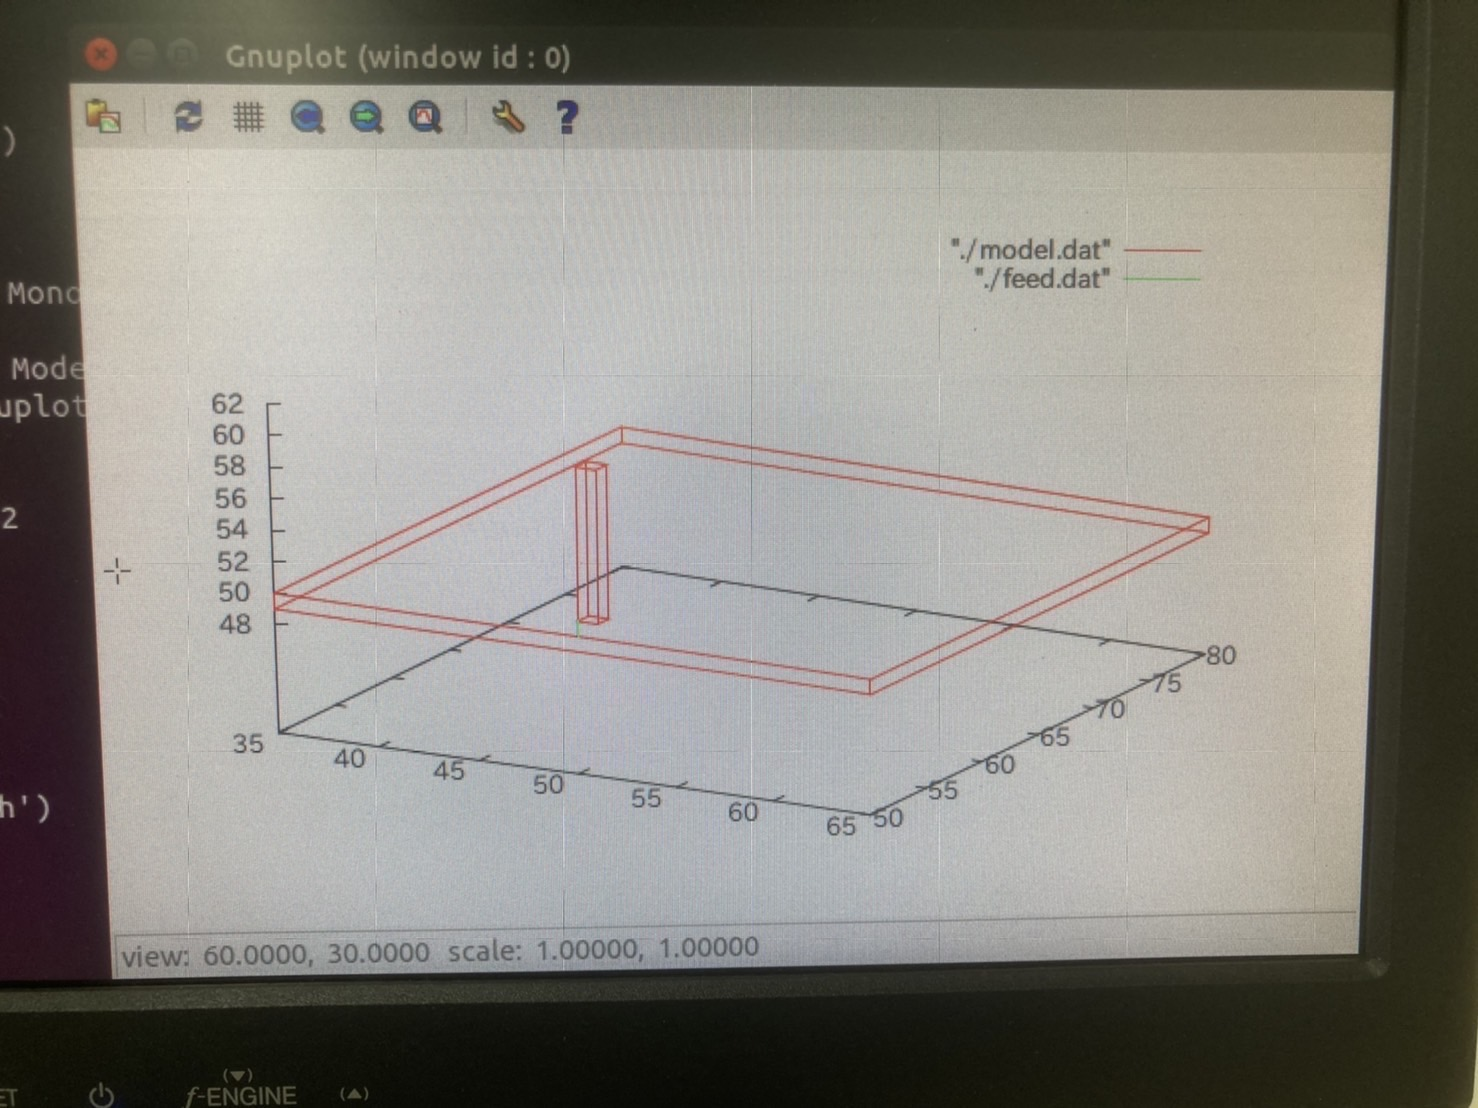
\includegraphics[keepaspectratio,scale=0.13]{pic1.JPG}
%     \end{center}
%     \caption{モデリング例1}
%   \end{minipage}
%   \begin{minipage}[b]{0.45\linewidth}
%   \begin{center}
%     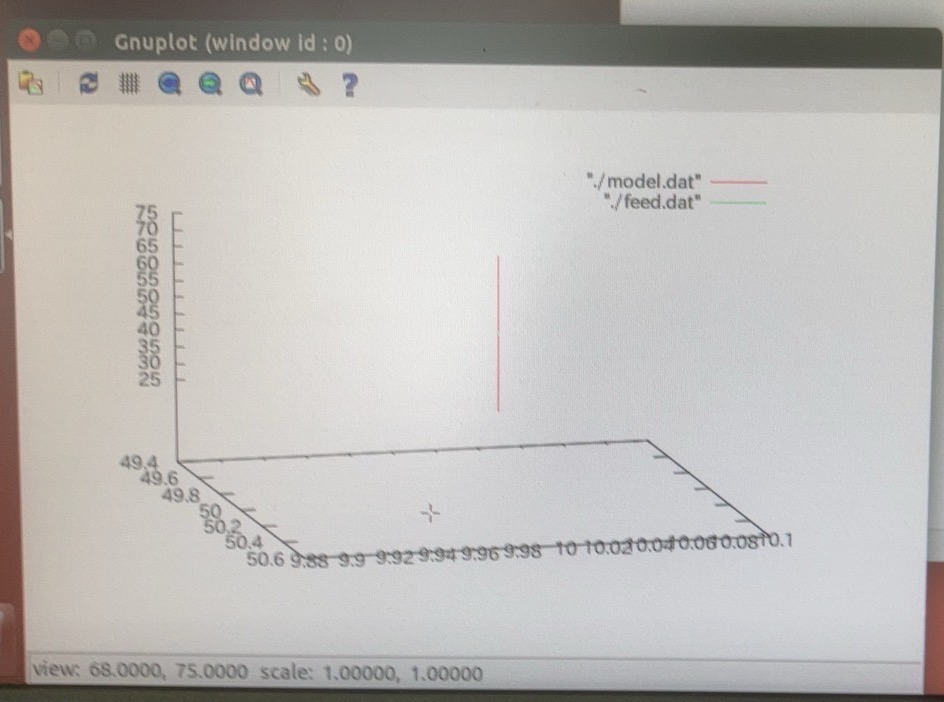
\includegraphics[keepaspectratio,scale=0.2]{pic2.JPG}
%     \end{center}
%     \caption{モデリング例2}
%   \end{minipage}
% \end{figure}

\section{実験の内容}

初めにダイポールアンテナを作成した。次にそのダイポールアンテナをもとに、
八木宇田アンテナを作成し、改良を重ねていった。

\subsection*{ダイポールアンテナ}

ダイポールアンテナを作成するに当たって、初めに素子の長さを決定する必要があった。
わたしたちの班では、多くの放送局が密集している周波数帯に合わせてアンテナを作成
するということになったので、VSWRの値が490MHz付近の地点で最も1に近づくように設計
した。実際に設計したダイポールアンテナを図1に示す。

\begin{figure}[h]
  \centering
  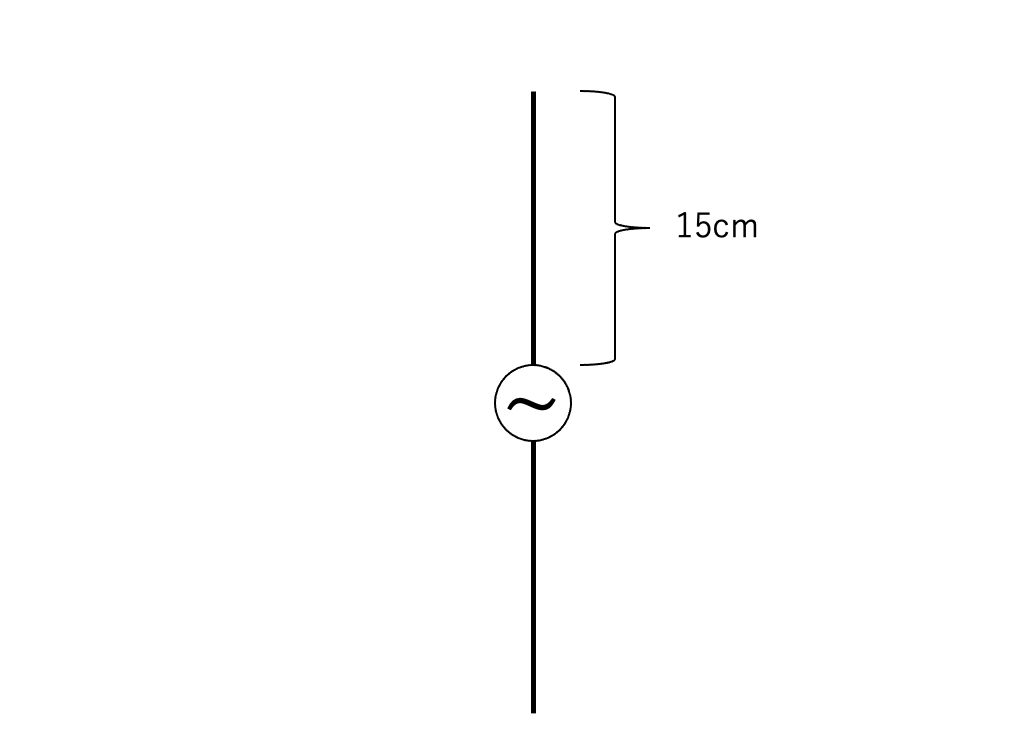
\includegraphics[scale=0.4]{pic3.png}
  \caption{作成したダイポールアンテナ}
\end{figure}

\subsubsection*{素子長}
素子の長さを決定するためにモデリングを複数回行ったところ、目的の周波数に対応する1/4波長
の素子長にすると、VSWRの値は目的の値よりも少し低いところで最も1に近づくことが確認できた。
この性質は初めにモデリングの練習で行った1GHzのダイポールアンテナのモデリング結果にも反映
されていることが確認できる(図2)。そのため、目的の周波数に対応する1/4波長よりも少し長めの
15cmつまりは500MHzに対応する長さとし、モデリングを行ったところ良好な値が得られたため、
この長さで作成することにした。実際のモデリングの結果を図3,4,5に示す。

\begin{figure}[h]
  \centering
  \begin{minipage}[b]{0.45\linewidth}
  \begin{center}
    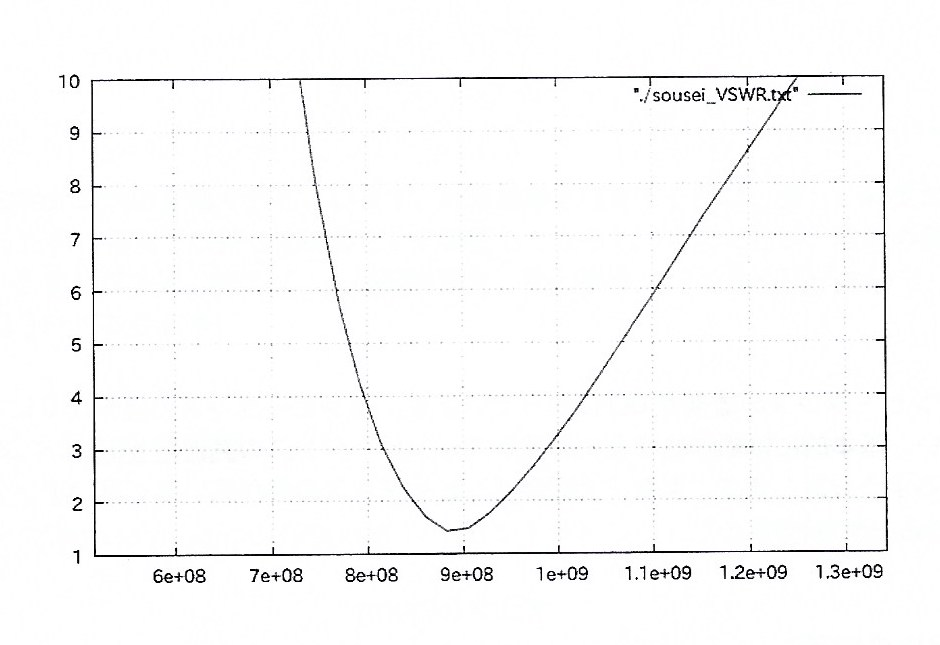
\includegraphics[keepaspectratio,scale=0.2]{pic6.jpeg}
    \end{center}
    \caption{テキストp.18より\\900MHzで最も近づく}
  \end{minipage}
  \begin{minipage}[b]{0.45\linewidth}
  \begin{center}
    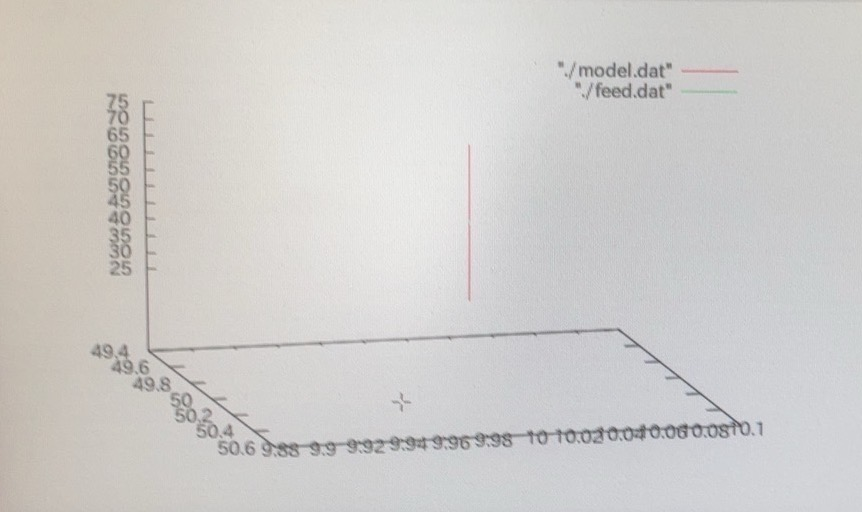
\includegraphics[keepaspectratio,scale=0.25]{pic9.jpg}
    \end{center}
    \caption{モデリング}
  \end{minipage}
\end{figure}

\begin{figure}[h]
  \centering
  \begin{minipage}[b]{0.45\linewidth}
  \begin{center}
    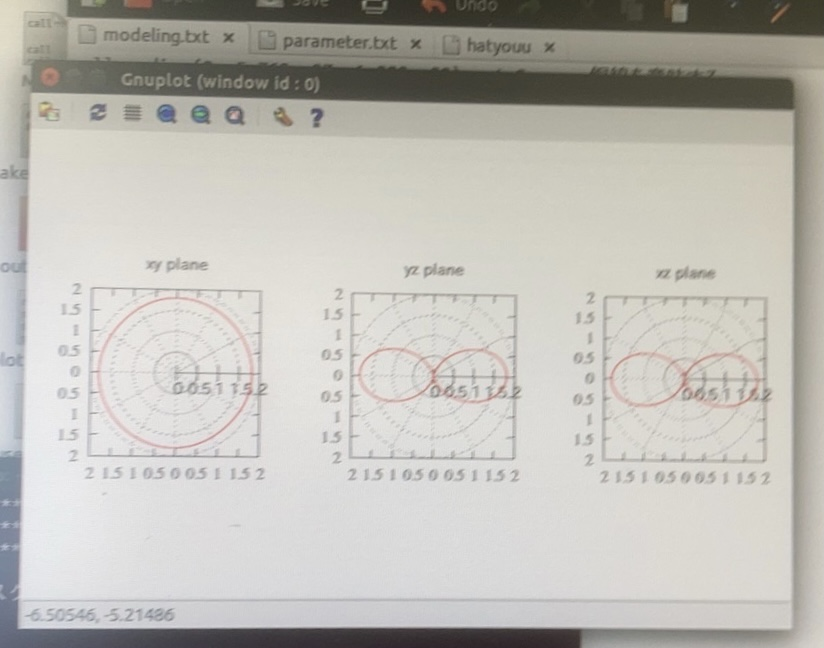
\includegraphics[keepaspectratio,scale=0.2]{pic8.jpg}
    \end{center}
    \caption{指向性}
  \end{minipage}
  \begin{minipage}[b]{0.45\linewidth}
  \begin{center}
    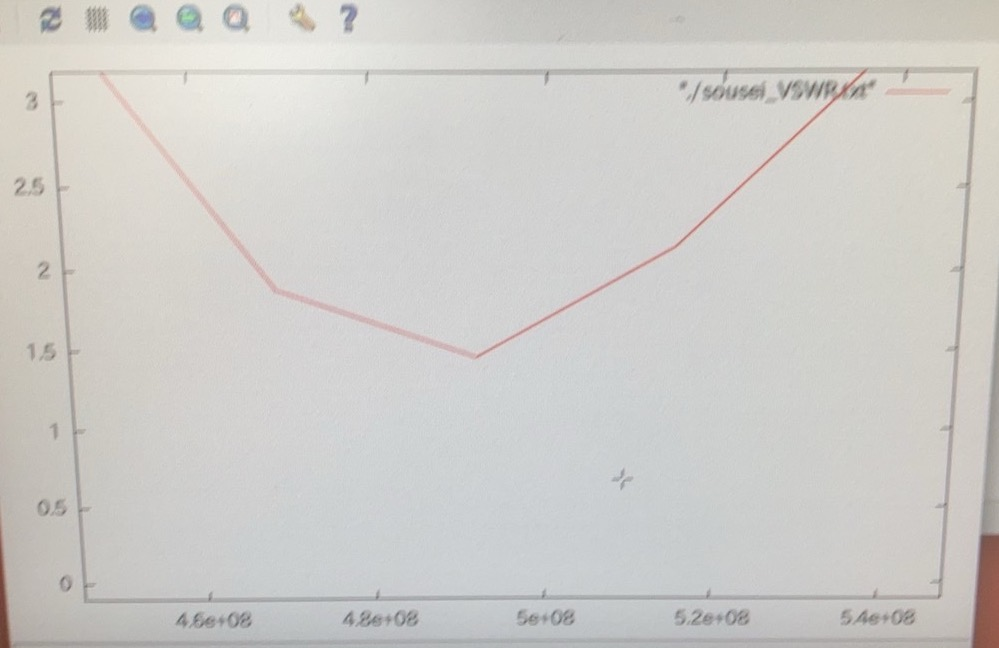
\includegraphics[keepaspectratio,scale=0.2]{pic7.jpg}
    \end{center}
    \caption{素子長150mmの時のVSWR}
  \end{minipage}
\end{figure}

\subsubsection*{計測結果}
実際にテレビに接続し、計測を行った結果は以下の表1のようになった。

\begin{table}[h]
  \centering
  \caption{ダイポールアンテナ 測定結果}
  \begin{tabular}{|l|l|l|l|l|l|l|}
  \hline
  NHK大津                     & NHK大阪                    & 琵琶湖放送                     & MBS                      & ABC                      & 関西テレビ                    & 読売テレビ                    \\ \hline\hline
  \multicolumn{1}{|c|}{5dB} & \multicolumn{1}{c|}{5dB} & \multicolumn{1}{c|}{11dB} & \multicolumn{1}{c|}{5dB} & \multicolumn{1}{c|}{4dB} & \multicolumn{1}{c|}{6dB} & \multicolumn{1}{c|}{4dB} \\ \hline
  \end{tabular}
  \end{table}

全体的に非常に良い数値を得ることができた。アンテナの設計上、NHK大津,琵琶湖放送は映り
ずらいと考えていたが、とても強い値を記録した。逆に、比較的映り安いと考えていた読売テレビ
が、少しだけ低い数値となった。

\subsection*{八木宇田アンテナ}
初めに作成したダイポールアンテナを放射器とする八木宇多アンテナを作成し、更なる性能
向上を図った。モデリングでは、指向性を一方向へ絞ることを目標に、様々な検証を行った。
八木宇田アンテナを選んだ理由としては、材料が準備しやすく、最も簡単に性能向上を図れる
と考えたからだ。

\subsubsection*{設計/モデリング}

まず初めに、テキストp.27を参考にし、反射器と放射器の距離を1/2波長(30cm)、放射器と
導波器の距離を1/4波長(15cm)として、モデリングを行った。モデリングを行ったものを図6に
示す。

\begin{figure}[h]
  \centering
  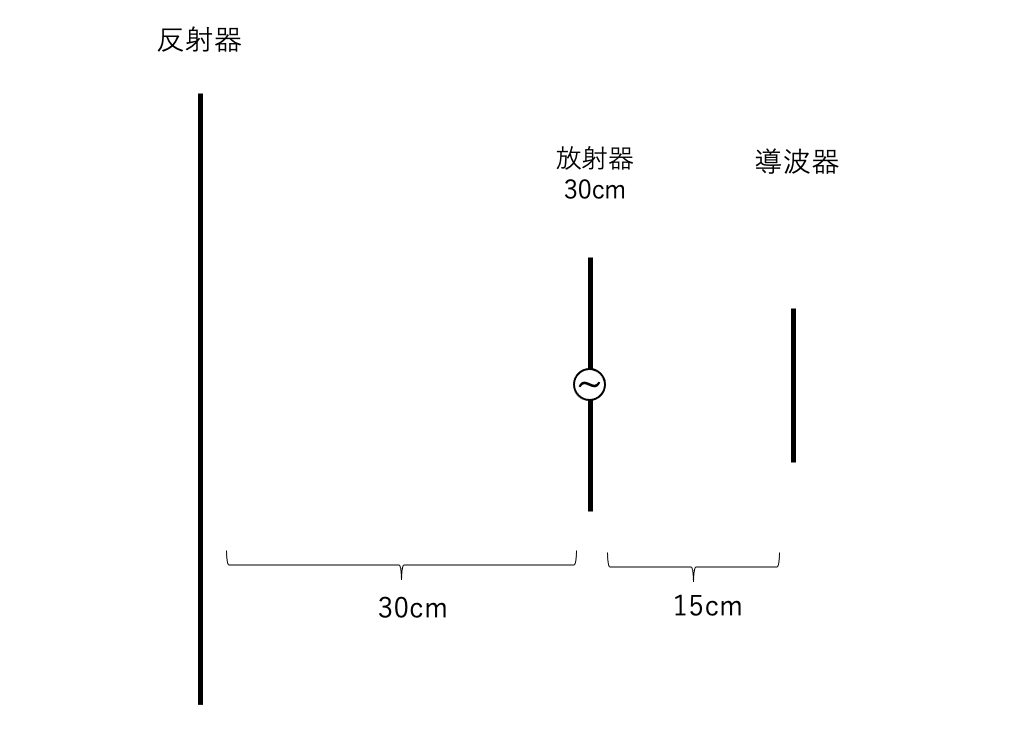
\includegraphics[scale=0.5]{pic5.png}
  \caption{}
\end{figure}

このアンテナのモデリング結果として得られたものが、反射機方向に指向性が出てしまっており、
求めてていたものとは大きく異なる結果となってしまった。その原因を明らかにしようと努力
したが、原因を特定するには至らなかった。\\
その後、様々な資料や教室に設置されていた八木宇田アンテナを観察し、素子間隔を全て
1/4波長にすること、モデリング通りの長さで反射器と放射器を作成することの二つを行うこと
とした。その時にモデリングを行ったものを図7,8,9,10に示す。

\begin{figure}[h]
  \centering
  \begin{minipage}[b]{0.45\linewidth}
  \begin{center}
    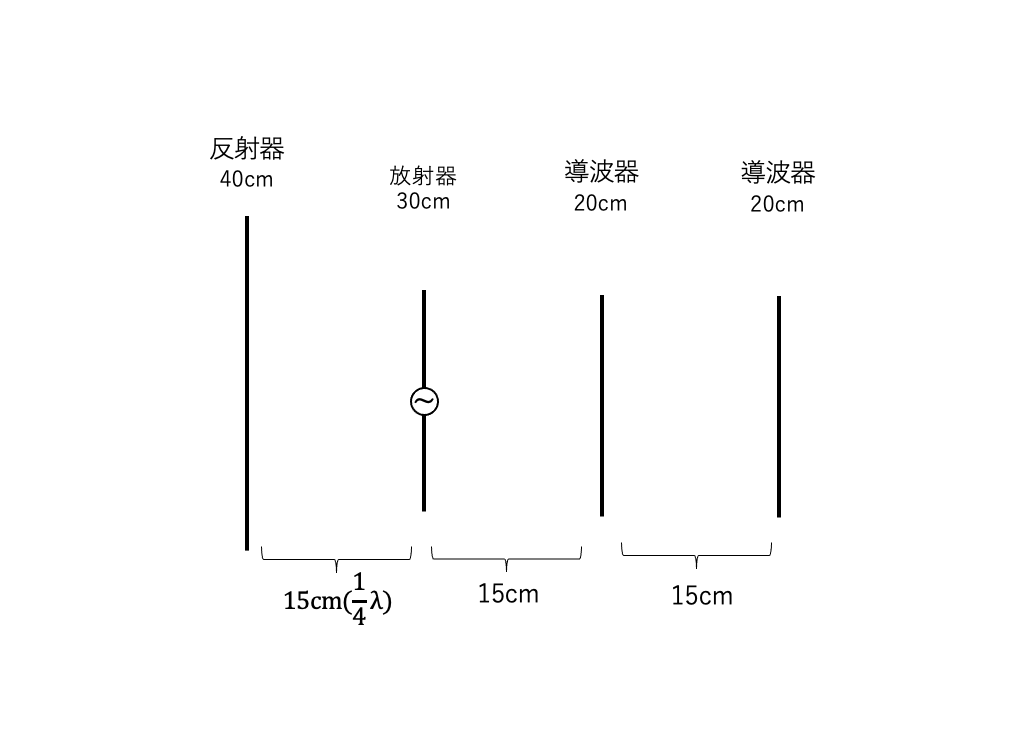
\includegraphics[keepaspectratio,scale=0.4]{pic4.png}
    \end{center}
    \caption{モデリング}
  \end{minipage}
  \begin{minipage}[b]{0.45\linewidth}
  \begin{center}
    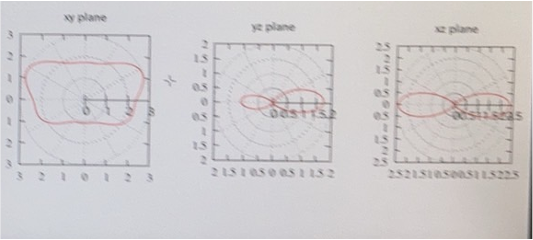
\includegraphics[keepaspectratio,scale=0.5]{pic10.png}
    \end{center}
    \caption{指向性}
  \end{minipage}
\end{figure}

\begin{figure}[h]
  \centering
  \begin{minipage}[b]{0.45\linewidth}
  \begin{center}
    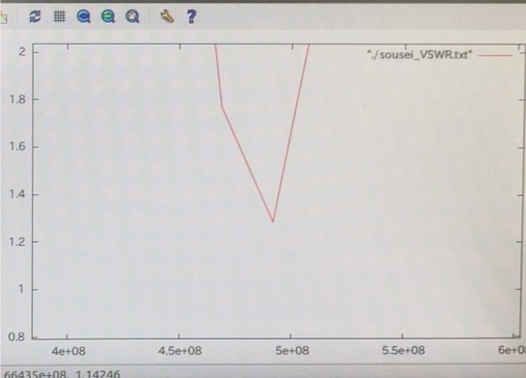
\includegraphics[keepaspectratio,scale=0.4]{pic11.png}
    \end{center}
    \caption{VSWR}
  \end{minipage}
  \begin{minipage}[b]{0.45\linewidth}
  \begin{center}
    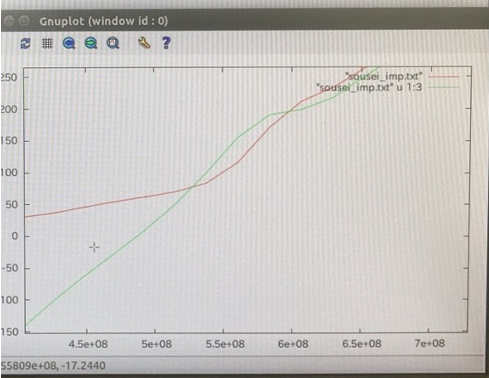
\includegraphics[keepaspectratio,scale=0.4]{pic12.png}
    \end{center}
    \caption{インピーダンス}
  \end{minipage}
\end{figure}
\newpage

指向性に着目すると、導波き方向へ指向性が出ていることが確認できる。また、
VSWRはダイポールアンテナに比べると限定的な周波数帯域に対して鋭く沈み込んでいる
ことも分かる。

\subsubsection*{計測結果}
実際にテレビに接続し、計測を行った結果は以下の表2のようになった。

\begin{table}[h]
  \caption{自作八木宇田アンテナ 測定結果}
  \centering
  \begin{tabular}{|l|l|l|l|l|l|l|}
  \hline
  NHK大津                     & NHK大阪                    & 琵琶湖放送                    & MBS                      & ABC                      & 関西テレビ                    & 読売テレビ                  \\ \hline\hline
  \multicolumn{1}{|c|}{1dB} & \multicolumn{1}{c|}{1dB} & \multicolumn{1}{c|}{5dB} & \multicolumn{1}{c|}{4dB} & \multicolumn{1}{c|}{2dB} & \multicolumn{1}{c|}{4dB} & \multicolumn{1}{c|}{×} \\ \hline
  \end{tabular}
  \end{table}

  ダイポールアンテに比べ全体的に数値が大きく落ち込んでしまった。読売テレビに関しては
  そもそも受診することすらできなくなってしまい、結果として改良は失敗となってしまった。

\section{考察}
八木宇多アンテナにしたことで性能が大きく下がってしまったことについての
考察を行う。モデリングを行った上で作成をしていることから、設計自体は間違い
ではなかったと仮定し、考察を行った。

\subsubsection*{放射器の歪みがもたらした可能性}

作成した八木宇田アンテナの放射器が前回のダイポールアンテを再利用している
こともあり、大きく歪みが発生し長さが短くなったことが考えられる。ここでは
ダイポールアンテナの片側に5mmの歪み、両側で10mmの歪みが発生したと考えると、
表3より。目標を490MHzとすると10mmで460MHzまで落ち込むことが確認できる。
460MHzはどの放送局も使用していない周波数帯域であるため、受信できなかったこと
にも納得がいく。さらに、この表はあくまで周波数であるので、実際は先ほども述べた
よう、目標の値よりも低い周波数帯域となることがわかっているので、それを加味すると
より、映らなかった原因なのではと考えた。

\begin{table}[h]
  \centering
  \caption{周波数と対応する1/4波長}
  \begin{tabular}{|c||c|c|c|c|c|c|}
  \hline
  周波数(MHz)  & 440    & 450   & 460    & 470    & 480 & 490    \\ \hline
  1/4波長(mm) & 170.25 & 166.5 & 162.75 & 159.25 & 156 & 152.75 \\ \hline
  \end{tabular}
  \end{table}

\subsubsection*{天気による影響}

自作アンテナの測定を行った日7月13日は雨が少し降る程度の天気であり、ダイポールアンテナの
測定を行った日はとても快晴の日であった。ここで考えられる原因が、天気による要因、
すなわちは水分による影響である。空中の水分、雲に含まれる水分などによって
電波の減衰が起こり、うまく受信できなかったのではと考えた。事実、この日は
周りの班もうまく受診できていないことが多かったことがわかっている。しかし、
このことを検証するには,電波塔が設置されている宇佐山のデータや、水分によって
どれだけ電波が減衰するかなど新たな調査が必要であり、さらには、先生は天気は
それほど影響しないとおっしゃっていたので、考察の域を出ることはないが、作成したアンテナ
がもとより高性能でなかったことを加味すると、やはり原因の一つではないかと
考えた。

\section{付録:各回のレポート}

\subsection*{6月22日}

先週に続き、アンテナの改良をおこなった。先週はアンテナの長さを読売テレビに
合わせ約15cm後半から16cmとし、計測をおこなったが、今週はもう一度モデリング
を行い長さ15cmから約14.5cmまで縮めることにした。15cmの時は、全てのチャン
ネルが写りまた全てのチャンネルで抵抗を入れても写った。その中でも、毎日にテレ
ビは8dBの抵抗下でも正確に写すことができた。しかし、読売テレビは3dB、ABCは
4dBとアンテナの長さが読売テレビよりなのにも関わらず、読売テレビはあまり強
い強度で受信できていないことがわかった。次にアンテナの長さを14.5cmと少し
だけ短くしてもう一度実験を行った。結果は15cmの時に比べて、全体的に高い抵
抗値でも正確にテレビを映すことができた。中でもBBCは11dBの抵抗でも映すこ
とができ、読売テレビも4dBの抵抗まで耐えられるようになった。しかし、ABCテ
レビは2dBの抵抗までしか映すことができなかった。アンテナの長さを短くし、よ
り写りやすくなると予想していたが、異なる結果が得られてしまった。しかそ、こ
の時は時間があまりなく、急ぎでの測定だったこともあるので、自習にもう一度測定
をし直し、もう一度結果がどうなるのかを確認したいところである。15cm,14.5c
mの二つの測定結果から得られる考察を上げる。まず琵琶湖放送,BBCは地元のチャ
ンネルでもあることから、非常に強い電波強度で受信できていると考えられる。1
cmの方では8dB,14.5cmの方では11dBの抵抗下でも正常に映すことができた。対
照的に、ABC,読売テレビは、アンテナの性能影響を、比較的大きく受けているこ
とから、琵琶湖放送に比べ弱い電波強度であることが考えられる。だが、実験を
行っていて、持つアンテナの場所や角度で映るかどうかが決まっていた節も見ら
れたので、実験環境ももう一度整備し直し、実験を行うことでより正確なデータ
を採取したい。

\subsection*{6月29日}

先週に続き、アンテナの改良を行った。今回は、折り返しアンテナ、八木・宇多ア
ンテナ、ダイポールアンテナの後ろに金属板を設置したアンテナのモデリングを行
った。ダイポールアンテナの後ろに金属板を設置したアンテナについては、適切な
モデリングができ、計算の数値も比較的適切なものが得られたが、八木・宇多アン
テナのモデリングが、モデリングを行うツールの補正機能によって適切なモデリン
グ結果が得られなかった。しかし、演算結果としては非常に良い結果が得られたた
め、実際に発布スチロールと銅線を利用して、八木・宇多アンテナのさくせいを行
った。導波器と反射器の長さは適当に行い、その二つの距離を測定し、八歩スチロ
ールに固定した。テレビに接続し、測定を行った結果、すべてのチャンネルで4dB
以上の抵抗下でも映ることができたが、この結果は初めに作成した、ダイポール
アンテナとほとんど一致するものであった。これは、八木・宇多アンテナを作成
したのにも関わらず、あまり良い指向性が得られていなかったからだと考えられ
る。そのため、指向性を得るためのモデリングや、折り返しアンテナの作成を再
来週以降行っていきたい。

\subsection*{7月6日}

授業時間内で、先生へ実験の進捗報告をした。また、最終発表会に向けてチーム内
で左まっざまな準備を行った。私たちのグループは、VGA接続端子を持つコンピュ
ータを保持する学生がいないので、紙を映し出す装置を用いて最終発表を行うこ
とにした。先生への報告時に私たちの作成した八木宇多アンテナの間違っている
点について指摘された。その内容としては、私たちのグループが作成した八木宇
多アンテナは、モデリング上の八木宇多アンテナとは大きく縮尺が異なっていた
ことだ。モデリング上で作成した八木宇多アンテナの導波器と反射器の長さと私
たちが作成したものは大きく異なっていた。そのためか、実験結果としては、ダ
イポールアンテナと大きく変わらないものが出来上がってしまったとわかった。
そのため私たちはTAさんからMatlabの使い方について教わり、次週の実験までに
理想の八木宇多アンテナの導波器と反射器の長さを見つけるように、モデリング
行うことにした。Matalabでのモデリング結果をもとに次週での実験でアンテナ
を完成まで持っていきたい。

\subsection*{7月13日}

先々週と先週に続き引き続き八木宇多アンテナの作成、改良を加えた。
Matlabでのモデリングが想定していたものより、大きく異なる値が出てしまったの
で、教室でもう一度モデリングを行うところから始めた。初めに行ったのは、先週
の進捗報告の際に先生に注意された点を改善した。内容としては、モデリングと作
成するアンテナの誤差を2mm以下にした方が良いというものだ。先々週作成した八
木宇多アンテナは、反射器と導波器の長さを適当にしていたため、そこを改善し
た。改善を行い、いざ実験室に行き、値の測定を行ったが、改善されるどころか
ダイポールアンテナの時よりも悪い数値を記録してしまった。しかし、周りの班
の多くも同様にアンテナの調子が悪かったこともあり、何らかの原因が考えられ
るが、その原因についてはまだ明らかになっていない。その次に行った改良は、
反射機と導波器の素子感覚を変更することだ、今まではテキストp27ページのも
のと同様に、反射機は二分の一波長、導波器は4分の1波長分離していたが、
インターネットなどを用いて改良法を詮索した結果、どちらも二分の一波長に
することにした、どちらも二分の一波長にしモデリングを行ったところ、今ま
でのものより、強い指向性を持っていることが発覚した。さらに、導波器の個
数を1個から2個にしたものについてもモデリングを行ったところ、より強い指
向性が確認できた。その後モデリングの内容にそい、全素子数4個の八木宇多
アンテナを作成し、実験室に行き測定を行った。結果は1回目の改良とほぼ同
様の結果が得られ、原因がよくわからないまま実験が終わってしまった。一
つ原因として考えられるのは、実験を重ねるたびに、放射器が少しずつ曲が
っていってしまったのではないかと考えた。また、あの日は雲も多く、雨も
降っており、天候がとても不安定であったことも何らかの原因ではな以下と
考えた。私たちが得た一つの教訓はテキストを鵜呑みにしてはいけずに、様
々な方向から物事を調べ、捉え、吸収することが大切だと学ぶことができた
。これは、テキスト通りに作ったことで、貴重な実験時間の一日を潰してし
まったからである。

\end{document}